% #############################################################################
% This is Chapter 4
% !TEX root = ../main.tex
% #############################################################################
% Change the Name of the Chapter i the following line
\fancychapter{Preliminary Results}
\cleardoublepage
% The following line allows to ref this chapter
\label{chap:implement}


\section{Poster Presented: Challenges in Methane Detection Using ML: A Critical Analysis and Research Agenda}

\subsection{Context and Motivation}

As part of the broader doctoral research on causal modeling and satellite-based environmental monitoring, a preliminary study was conducted to critically assess the current state of methane detection methodologies leveraging satellite imagery and machine learning (ML). This exploratory work emerged during the initial phase of literature review and methodological mapping, aiming to establish a strong conceptual foundation for the subsequent development of a causal modeling framework for methane dynamics.

Although not the central axis of the thesis, this subcomponent produced a valuable standalone contribution and was selected for presentation at the \href{https://www.atmos2024.org/}{ATMOS 2024} conference, organized by the European Space Agency (ESA) under the EO Science for Society Programme Element. The event took place in Bologna, Italy, from July 1--5, 2024, and gathered the scientific community working with atmospheric Earth observation data. The poster was accepted as part of the conference’s track on methane monitoring and artificial intelligence applications in Earth Observation (EO).

\subsection{Poster Title and Scientific Contribution}

This study delivered a systematic analysis of recent efforts in methane detection from EO data, highlighting common challenges across published works and establishing key gaps in reproducibility, data availability, and methodological transparency. While the full poster is provided in Appendix~\ref{chapter:appendixA}, the study reviewed:

%\textbf{Title:} Navigating the Challenges in Methane Detection Using ML: A Critical Analysis and Research Agenda.
%\textbf{Authors:} Marco Rueda, Prof. Dr. Rodrigo Ventura, Dr. Miguel Arana-Catania, Dr. David R. Ardila.

\begin{itemize}
    \item The diversity and fragmentation in publicly available satellite datasets for methane detection.
    \item The limited reproducibility and code accessibility within the field, where approximately 45\% of reviewed studies either lacked public data or included major caveats to their use.
    \item The inconsistent application of modern ML standards such as robust cross-validation, explainability, and uncertainty estimation.
\end{itemize}

While some positive trends were observed, such as a gradual increase in code sharing and documentation, the poster underscored that the field lacks standardized benchmarks and unified data pipelines for ML-based methane detection.

\subsection{Relevance to the Thesis}

Although this is not the principal line of research pursued in the dissertation, the presented work is strategically relevant for two reasons. First, it validates the scientific necessity of the thesis’ core research problem: the need for reproducible, scalable, and causally sound models to interpret atmospheric methane dynamics. Second, it frames the importance of integrating ML best practices with high-quality EO data sources, including those used in this dissertation (e.g., TROPOMI and MODIS). 

This analysis has directly informed the construction of data pipelines, the selection of benchmark regions and datasets, and the design of the proposed causal inference framework described in later sections.

\subsection{Position within the ESA ATMOS24 Conference}

The ESA ATMOS 2024 conference provided a timely venue to disseminate this early finding. The event’s scientific objectives, particularly the focus on integrating artificial intelligence with Earth observation and fostering large-scale R\&D initiatives, aligned closely with the themes addressed by the poster. The poster was well received and contributed to broader discussions around open science, multi-mission synergy, and the design of next-generation atmospheric retrieval algorithms.

\subsection{Recommendations and Research Agenda}

Based on the review, the poster formulated a preliminary research agenda which complements this thesis’ long-term objectives:

\begin{enumerate}
    \item \textbf{Benchmarking:} Promote the development of shared, validated benchmark datasets for training and testing ML models for atmospheric methane detection.
    \item \textbf{Data Integration:} Advocate for the synthesis of multi-source EO datasets (e.g., TROPOMI, OCO-2, MODIS) into harmonized spatial-temporal formats suitable for ML applications.
    \item \textbf{Transparent ML Workflows:} Encourage adoption of reproducible ML pipelines that include public codebases, robust validation, and performance reporting across multiple geographies and seasons.
\end{enumerate}

These directions are closely aligned with the strategic vision of ESA’s EO program and serve to guide both the scientific community and future work in this thesis.

\subsection{Conclusion}

The poster presented at ATMOS 2024 represents a foundational, yet independent, contribution to the broader research effort. While preliminary, it offered an evidence-based critique of current practices and provided valuable inputs for the methodological development of this dissertation. It also reinforced the strategic alignment between the dissertation's objectives and the priorities outlined by the European EO community.


%%%%%

\section{Testing our Causal Analysis Framework}

Early experiments have been conducted to validate our framework on benchmark datasets and synthetic examples. These preliminary results demonstrate the robustness of our approach and guide further development.

\subsection{Case 1 (Time Series Correlation)}
The dataset, originally used in the tutorial by Venugopal et al.~\cite{Venugopal2023}, consists of synchronized behavioural time series extracted from a controlled observational study. It contains $n = 5,229$ equally spaced samples, with two primary continuous variables: \texttt{S1\_Joy} and \texttt{S2\_Joy}. These variables quantify the smiling intensity of two individuals over time, expressed as normalized evidence scores derived from facial expression recognition algorithms. Sampling was performed at a fixed frame rate (approximately 30~Hz), yielding a temporal resolution suitable for sub-second lag analysis.  

Missing values are present at scattered points, primarily due to transient occlusions or detection dropouts, and are handled via linear interpolation before correlation or causality computations. The two time series are stored in a CSV file \texttt{synchrony\_sample.csv}, with each column representing one subject’s measurements and each row corresponding to a sequential time frame.  

The dataset is particularly appropriate for correlation and causality tests because:  
(i) both series are continuous, bounded in $[0,1]$, and comparable in scale;  
(ii) temporal alignment is precise, enabling valid lag-based measures such as time-lagged cross-correlation (TLCC); and  
(iii) the behavioural nature of the signals makes them ideal for demonstrating cases where correlation and causality diverge.  

Using this public time-series dataset of 5,229 samples, we replicated an analysis by Venugopal et al.~\cite{Venugopal2023}. The original study computed Pearson correlation, TLCC, and Dynamic Time Warping distances to establish baseline associations. We confirmed those correlation measures as expected. We then extended the analysis with causal tests, applying Granger causality and transfer entropy on the same dataset. The results successfully reproduced known patterns and provided new insights. For instance, some variable pairs with high correlation showed no Granger causality (implying the correlation was non-directional or confounded), whereas others exhibited a clear causal direction that simple correlation could not detect. This not only validates our implementation of causality algorithms but also highlights their added value over traditional correlation analysis.  

\subsection{Case 2 (Granger Causality)}
We reproduced a classic econometric example using a Kaggle dataset of approximately 200 samples, examining whether advertising expenditures cause sales outcomes~\cite{Regi2023}. The dataset, \texttt{Advertising Budget and Sales.csv}, contains monthly observations of two main continuous variables: \texttt{TV Ad Budget (\$)} and \texttt{Sales (\$)}. Both are measured in US dollars, with the advertising budget representing the monthly expenditure on television advertising for a single product line, and sales representing the corresponding monthly revenue. Sampling is uniform in time, making the dataset suitable for time-series analysis without temporal resampling.  

Data preprocessing included selecting the two variables of interest and normalizing each series by its initial value to facilitate interpretability and remove scale effects in the Granger causality test. The resulting normalized series are dimensionless and maintain their temporal dynamics intact.  

The original analysis found a Granger causal relationship from TV advertising budget to product sales with a $p$-value of approximately 0.04, while the reverse (sales causing ad budget) yielded $p \approx 0.075$. Our re-analysis matched these findings but clarified the interpretation: the $p = 0.075$ pertains to the null hypothesis that ``sales do not Granger-cause advertising budget'', failing to reject this means, correctly, that there is no evidence that sales influence the budget, while advertising appears to influence sales.  

This exercise served as a sanity check for our causality code and reinforced the need for precise interpretation of Granger test results. The outcome increased our confidence in using Granger tests for more complex methane data, since the procedures behaved as expected on known, well-structured econometric data.


\subsection{Synthetic Data Test}
We generated a synthetic dataset (100 samples, 6 variables) designed to resemble features of our real problem, including autocorrelations and a mixed causal structure. In this controlled scenario, we assigned known causal links and incorporated both linear and nonlinear dependencies. An initial run of our pipeline revealed some misclassifications, particularly, several nonlinear causal links were missed when using linear tests alone. This prompted refinement of our linearity assessment heuristic.

To address this, we introduced a new metric, the MI/R$^2$ ratio (mutual information divided by the $R^2$ of a linear fit), to flag relationships that are highly dependent (high mutual information) but poorly explained linearly (low $R^2$). Using this metric, we could selectively apply nonlinear tests (like transfer entropy) in addition to linear Granger tests. After refining the pipeline, the synthetic dataset’s causal graph was recovered with 100\% accuracy, all true causal links were detected and no false links were introduced.

Figure~\ref{fig:synthetic} visualizes these findings, showing both the scatter plots and key metrics for two representative relationships: A~$\rightarrow$E (linear) and A$\rightarrow$F (nonlinear). Notably, the MI/$R^2$ ratio for A$\rightarrow$~F is extremely high, confirming that this relationship is nonlinear and poorly captured by linear models.

\begin{figure}[h!]
    \centering
    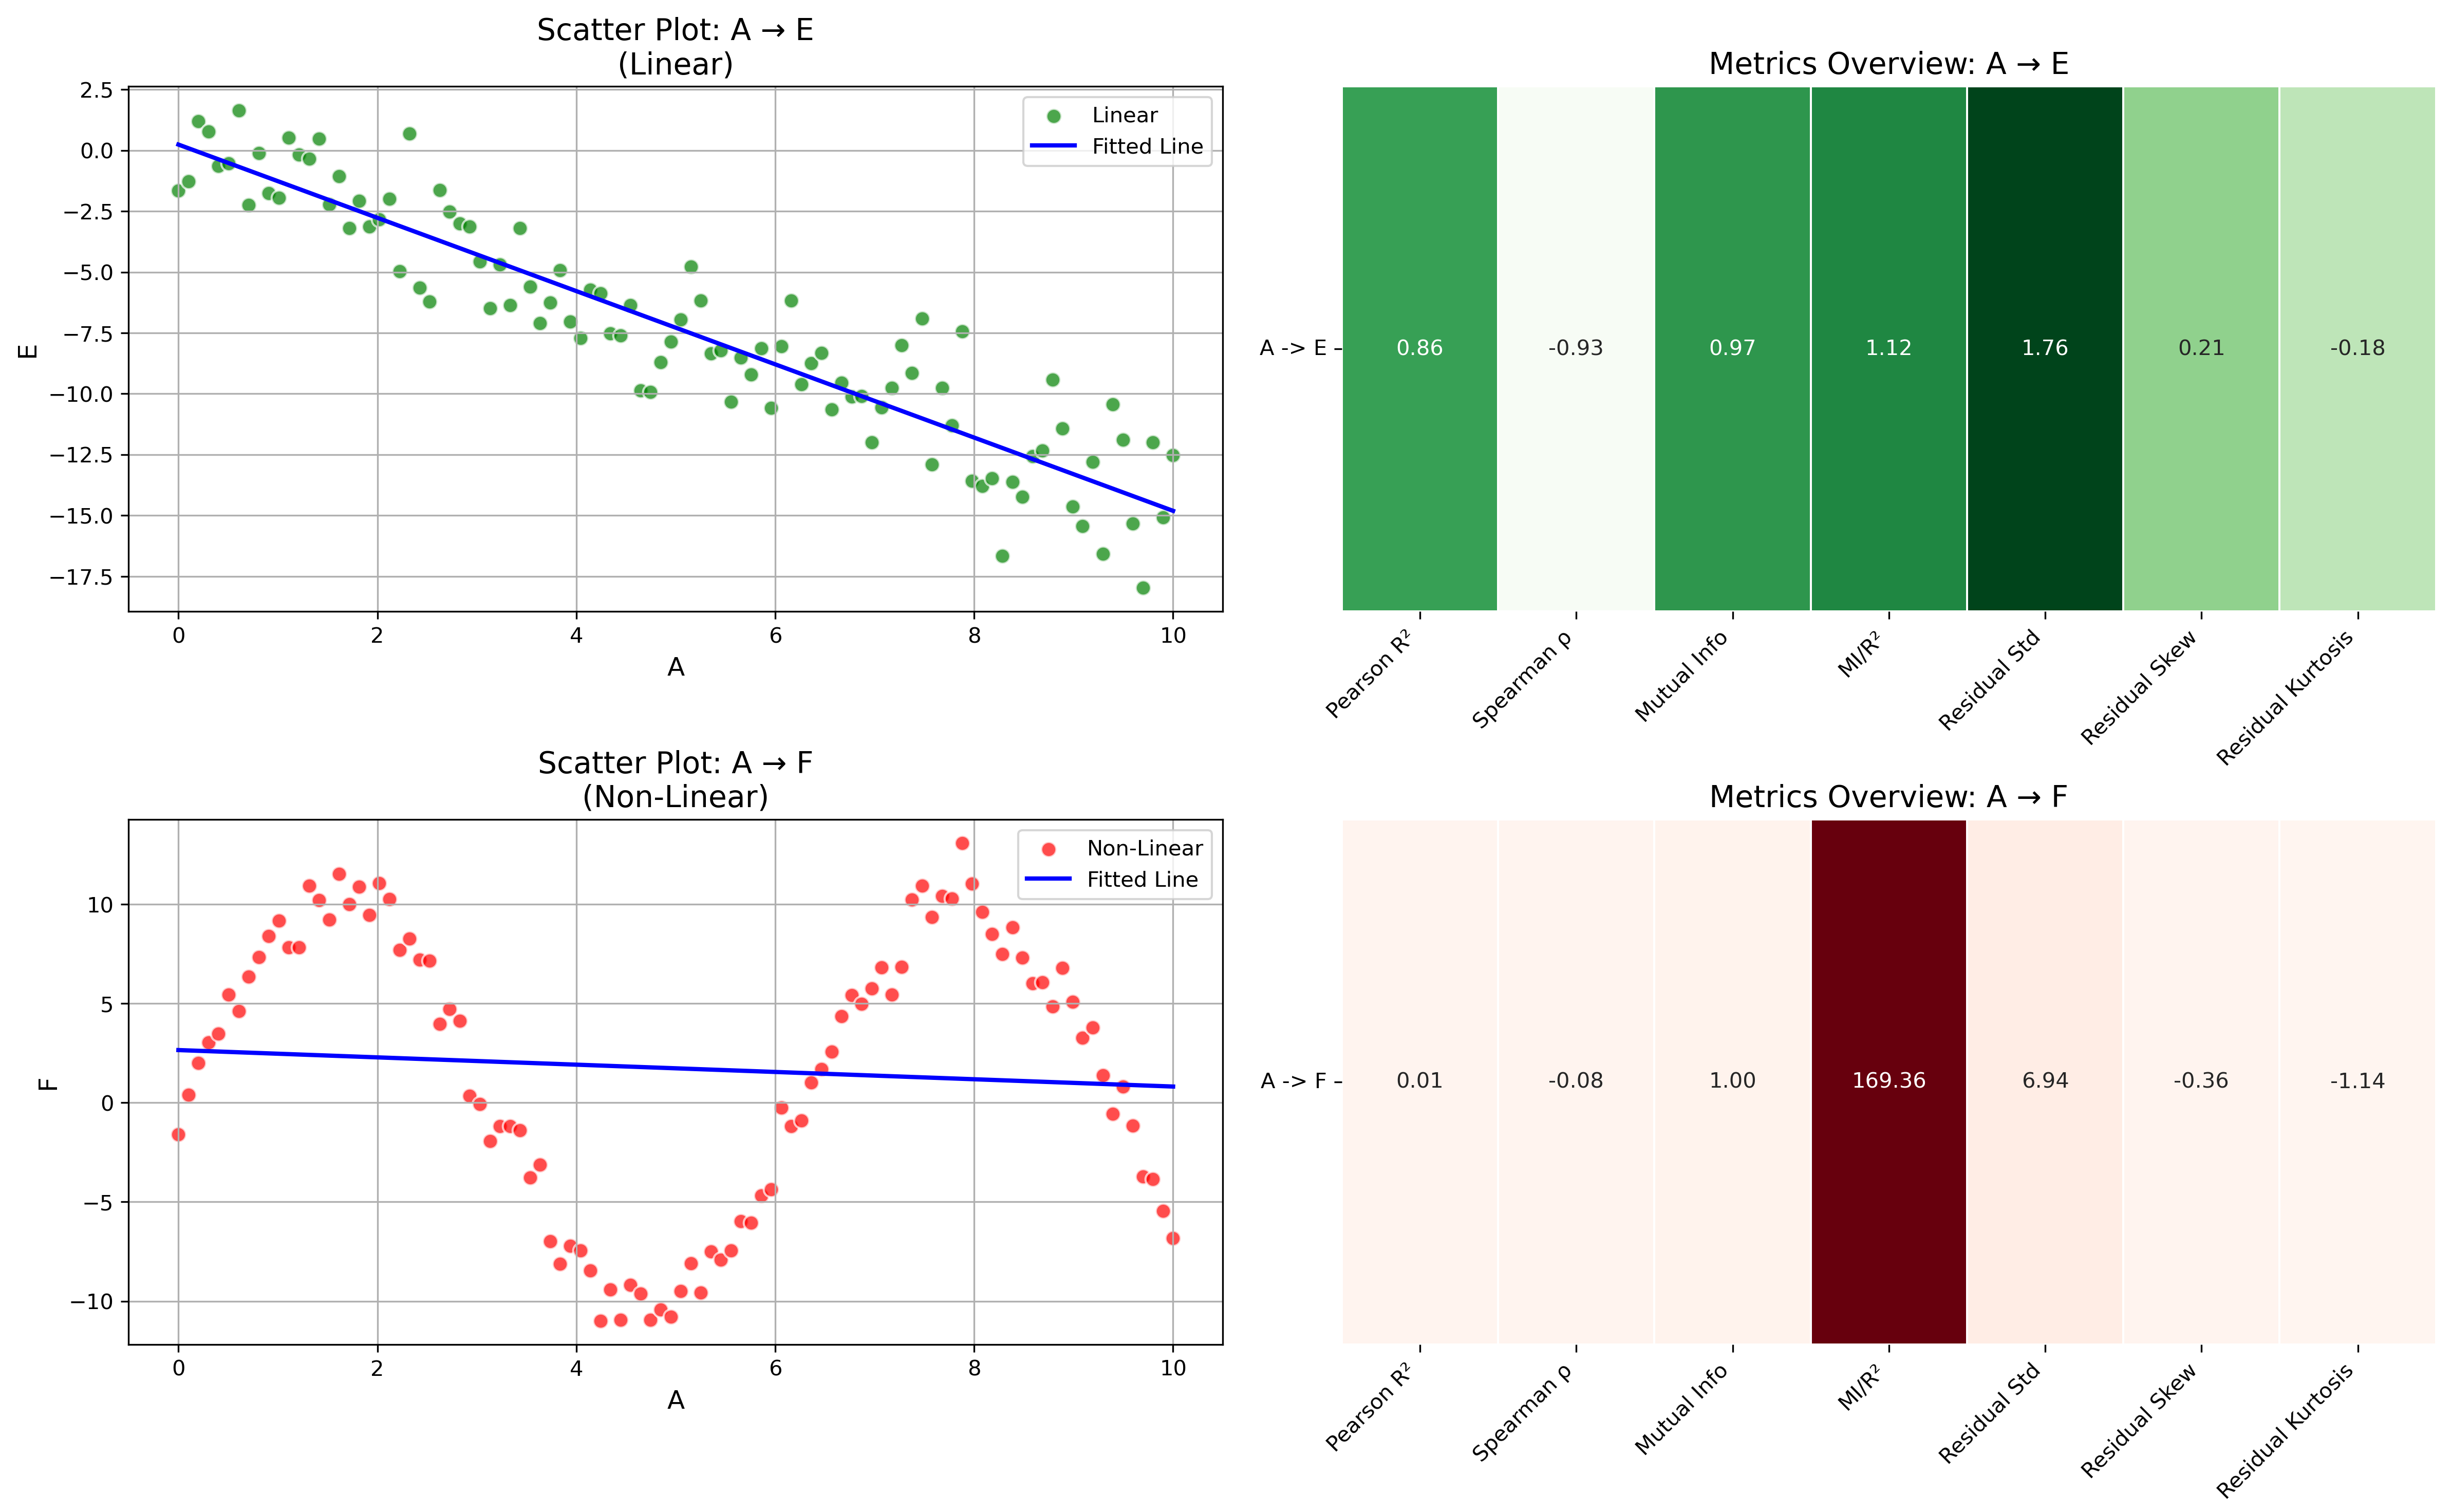
\includegraphics[width=0.8\textwidth]{Images/linearity_visualization.png}
    \caption[Linearity analysis of synthetic causal links]{\textbf{Linearity assessment and metric diagnostics for synthetic data.} Higher MI/R$^2$ values indicate greater nonlinearity. Left: Scatter plots show the relationships A $\rightarrow$ E (linear) and A $\rightarrow$ F (nonlinear), along with fitted linear regression lines. 
    Right: Associated metrics include Pearson and Spearman correlation, mutual information (MI), MI/$R^2$, and residual diagnostics. The MI/$R^2$ ratio is much higher for A $\rightarrow$ F, indicating a highly nonlinear dependence.}
    \label{fig:synthetic}
\end{figure}
    
These preliminary tests on benchmark and synthetic data validate our framework’s correctness and robustness. They also yielded valuable lessons. For instance, we confirmed the necessity of multiple comparison corrections, spurious links appeared before FDR control but vanished afterward, reinforcing the importance of statistical rigor. Additionally, while the Kaggle cases are not domain-specific to methane, they demonstrate that our tools generalize well and produce interpretable, plausible results.

\section{Reproducing the Baseline Paper Results (Ongoing)}
Encouraged by these results, we have begun applying our framework to actual methane remote sensing data. We are currently reproducing the analysis by Karoff and Vara-Vela~\cite{Karoff2023} on atmospheric methane concentrations as a function of geographic location, land cover type, and season. Using the full TROPOMI XCH$_4$ record (2017–2020) alongside land cover data, our scripts compute methane distributions and causal relations across land cover classes.

Initial findings align with the original study’s results. For example, croplands tend to exhibit the highest mean XCH$_4$ levels, shrublands the lowest, and wetlands, somewhat unexpectedly, show low concentrations in certain regions~\cite{Karoff2023}. Our causal analysis is investigating potential explanations: preliminary evidence suggests that variability in temperature and soil moisture may mediate the wetland–methane relationship, potentially explaining the lower-than-expected methane levels in wetland-rich zones.

Once this reproduction is complete, we will have a strong validation that our framework not only functions in theoretical and controlled settings, but also performs reliably on real-world Earth observation data. This will set the stage for the full causal analysis to be conducted on a global methane monitoring scale.

%%%%%